\documentclass[14pt, a4paper,reqno]{article}
\usepackage{hyperref}
\usepackage[warn]{mathtext}
\usepackage[utf8]{inputenc}
\usepackage[T2A]{fontenc}
\usepackage[russian]{babel}
\usepackage{amssymb, amsmath, multicol}
\usepackage{graphicx}
\usepackage[shortcuts,cyremdash]{extdash}
\usepackage{wrapfig}
\usepackage{gensymb}
\usepackage{floatflt}
\usepackage{lipsum}
\usepackage{verbatim}
\usepackage{concmath}
\usepackage{euler}
\usepackage{xcolor}
\usepackage{etoolbox}
\usepackage{fancyhdr}
\usepackage{subfiles}
\usepackage{enumitem}
\usepackage{amsthm}
\usepackage{indentfirst}
\usepackage{import}
\usepackage{multirow}
\usepackage{hhline}
\usepackage{calrsfs}

\DeclareMathOperator{\sign}{sign}

\RequirePackage[ left     = 1cm,
                 right    = 1cm,
                 top      = 2.0cm,
                 bottom   = 1.25cm,
                 includefoot,
                 footskip = 1.25cm ]{geometry}
                 
\setlength{\parskip}{ .5em plus .15em minus .08em }
\renewcommand {\baselinestretch}{ 1.07 }

\fancyhf{} % clear existing header/footer entries

\renewcommand{\footrulewidth}{ .0em }
\fancyfoot[C]{\texttt{\textemdash~\thepage~\textemdash}}

\makeatletter
\patchcmd\l@section{%
  \nobreak\hfil\nobreak
}{%
  \nobreak
  \leaders\hbox{%
    $\m@th \mkern \@dotsep mu\hbox{.}\mkern \@dotsep mu$%
  }%
  \hfill
  \nobreak
}{}{\errmessage{\noexpand\l@section could not be patched}}
\makeatother
\parindent = 1cm % отступ при красной строке⏎
\pagestyle{fancy}    
\renewcommand\qedsymbol{$\blacksquare$}

\newcommand{\when}[2]{
  \left. #1 \right|_{#2} \hspace
}
\renewcommand{\kappa}{\varkappa}
\RequirePackage{caption2}
\renewcommand\captionlabeldelim{}
\newcommand*{\hm}[1]{#1\nobreak\discretionary{}

\DeclareSymbolFont{T2Aletters}{T2A}{cmr}{m}{it}
{\hbox{$\mathsurround=0pt #1$}}{}}
% Цвета для гиперссылок
\definecolor{linkcolor}{HTML}{000000} % цвет ссылок
\definecolor{urlcolor}{HTML}{799B03} % цвет гиперссылок
 
\hypersetup{pdfstartview=FitH,  linkcolor=linkcolor,urlcolor=urlcolor, colorlinks=true}

\begin{document}

% НАЧАЛО ТИТУЛЬНОГО ЛИСТА
\begin{center}
  {\small ФЕДЕРАЛЬНОЕ ГОСУДАРСТВЕННОЕ АВТОНОМНОЕ ОБРАЗОВАТЕЛЬНОЕ\\ УЧРЕЖДЕНИЕ ВЫСШЕГО ОБРАЗОВАНИЯ\\ МОСКОВСКИЙ ФИЗИКО-ТЕХНИЧЕСКИЙ ИНСТИТУТ\\ (НАЦИОНАЛЬНЫЙ ИССЛЕДОВАТЕЛЬСКИЙ УНИВЕРСИТЕТ)\\ ФИЗТЕХ-ШКОЛА РАДИОТЕХНИКИ И КОМПЬЮТЕРНЫХ ТЕХНОЛОГИЙ}\\
  \hfill \break
  \hfill \break
  \hfill \break
  \Huge{Работа 3.2.8. \\ Релаксационные колебания}\\
\end{center}

\hfill \break
\hfill \break
\hfill \break
\hfill \break
\hfill \break
\hfill \break
\hfill \break
\hfill \break

\begin{flushright}
  \normalsize{Работу выполнил:}\\
  \normalsize{\textbf{Долгов Александр Алексеевич, группа Б01-106}}\\
\end{flushright}

\vspace*{\fill} %

\begin{center}
  \normalsize{\textbf{Долгопрудный, 2022}}
\end{center}

\thispagestyle{empty} % выключаем отображение номера для этой страницы

% КОНЕЦ ТИТУЛЬНОГО ЛИСТА

\newpage
\thispagestyle{plain}
\tableofcontents
\thispagestyle{plain}
\newpage
\section{Аннотация}

    В данной работе исследуются релаксационные колебания, возбуждаемые в электрическом контуре, состоящем
    из конденсатора, резистора и газоразрядного диода с S-орбразной вольт-амперной характеристикой.

\section{Теоретические сведения}

    \textbf{Автоколебания} - колебания, потери энергии в процессе которых периодически компенсируются
    постоянным источником энергии; система, в которой возможны автоколебания, называется
    \textbf{автоколебателной системой}. В отличие от вынужденных колебаний форма и период автоколебаний
    определяются свойствами самой системы, а не источника энергии.

    \subsection{Рассмотрение вырожденной автоколебательной системы}

    Автоколебательная система, не содержащая одного из накопителей колебательной энергии (конденсатора
    или катушки индуктивности), называется \textbf{вырожденной}. В качестве вырожденной автоколебательной
    системы рассмотрим цепь (см. рис. 1), содержащую источник постоянного напряжения $U$, ёмкость $C$, резистор $R$
    и нелинейный элемент с $S$-образной вольт-амперной характеристикой $I_S(U)$ (см. рис. 2).

    В данной работе в качестве такого нелинейного элемента выступает газоразрядный диод (газоразрядная лампа).
    При малых напряжених лампа практически не пропускает ток (участок 0da). Ток в ней возникает
    только в том случае, если разность потенциалов на её электродах достигает напряжения зажигания
    $U_1$. При этом скачком (участок ab) устанавливается конечная сила тока - в лампе возникает
    нормальный тлеющий разряд. При дальнейшем незначительном увеличении напряжения сила тока заметно
    возрастает по закону, близкому к линейному.

    \begin{minipage}{0.49\linewidth}
        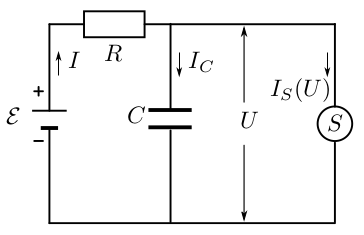
\includegraphics[width = \linewidth]{images/picture_1.png}
        \captionof{figure}{Вырожденная автоколебательная цепь}
    \end{minipage}
    \hfill
    \begin{minipage}{0.49\linewidth}
        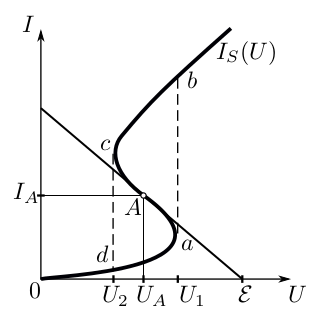
\includegraphics[width = \linewidth]{images/picture_2.png}
        \captionof{figure}{S-образная ВАХ}
    \end{minipage}

    Такая цепь описывается системой уравнений:
    \begin{equation*}
        \begin{cases}
            \mathcal{E} = IR + U \\
            I = I_C + I_S(U) \\
            I_C = C\dot{U}
        \end{cases}
    \end{equation*}
    Следовательно:
    \begin{equation}\label{eq}
        \mathcal{E} - U = (C\dot{U} + I_S(U))R
    \end{equation}
    В стационарном режиме, когда $\dot{U} = 0$, должно выполяться равенство:
    \begin{equation}\label{stationary_state}
        I_S(U) = \frac{\mathcal{E} - U}{R}
    \end{equation}
    График уравнения \eqref{stationary_state} представляет собой нагрузочную кривую, точки пересечения
    которой с ВАХ определяют стационарные состояния системы. Подберём параметры $\mathcal{E}$ и $R$ так,
    чтобы стационарное состояние $A(U_A, I_A)$ лежало на падающей ветви ВАХ. Покажем, что это состояние
    может быть неустойчивым. Зададим малое приращение $\Delta U$ в точке $U_A$ ($U(t) = U_A + \Delta U(t)$) и 
    представим в линейном приближении по $\Delta U$ ВАХ $I_S(U)$ вблизи состояния A:
    \begin{equation*}
        I_S(U_A + \Delta U) \approx I_S(U_A) + I_S^{'}\Delta U,
    \end{equation*}
    где $I_S^{'} = \frac{dI_S}{dU}\bigg|_{U = U_A}$. Подставим последнее соотношение в \eqref{eq}:
    \begin{equation*}
        \mathcal{E} - U_A - \Delta U = \left(C\frac{d(U_A + \Delta U)}{dt} + I_S(U_A) + I_S^{'}\Delta U\right)R
    \end{equation*}
    Также воспользуемся \eqref{stationary_state}:
    \begin{equation*}
        \mathcal{E} - U_A - \Delta U = \left(C\frac{d(\Delta U)}{dt} + \frac{\mathcal{E} - U_A}{R} + I_S^{'}\Delta U\right)R
    \end{equation*}
    \begin{equation*}
        -\Delta U = RC\frac{d(\Delta U)}{dt} + I_S^{'}R\Delta U
    \end{equation*}
    \begin{equation*}
        \frac{d(\Delta U)}{dt} + \frac{1 + I_S^{'}R}{RC}\Delta U = 0
    \end{equation*}
    Последнее уравнение - линейное однородное дифференциальное уравнение первого порядка. Его общее 
    решение имеет вид:
    \begin{equation*}
        \Delta U(t) = \Delta U(0) \exp\left(-\frac{1 + I_S^{'}R}{RC}t\right)
    \end{equation*}
    Из зависимости $\Delta U(t)$ видно, что при условии:
    \begin{equation}\label{condition}
        I_S^{'} < -\frac{1}{R}
    \end{equation}
    возмущение $\Delta U$ экспоненциально возрастает $\implies$ найденное стационарное состояние 
    действительно неустойчиво.

    При выполнении условий неустойчивости система совершает релаксационные автоколебания. Их траектория
    на рис. 2 являетя замкнутой и состоит из участков $da$ и $bc$ вольт-амперной характеристики между
    напряжениями $U_1$ и $U_2$, соединённых двумя вертикальными участками $ab$ и $cd$ (показаны штрихованными)
    линиями.

    \subsection{Описание колебаний}

    \begin{center}
        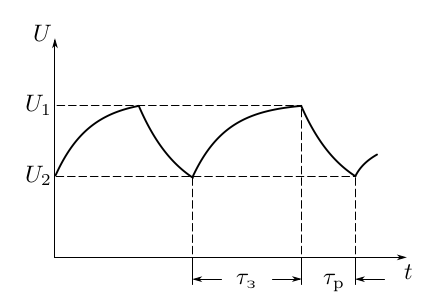
\includegraphics[width=0.5\textwidth]{images/picture_3.png}
        \captionof{figure}{Осциллограмма релаксационных колебаний}
    \end{center}
    
    Пусть в начальный момент напряжение на конденсаторе равно $U_2$. При зарядке конденсатора через резистор $R$ 
    напряжение на нём увеличивается. Как только оно достигает напряжения зажигания $U_1$, лампа начинает
    проводить ток, что сопровождается разрядкой конденсатора, поскольку источник тока, подключенный
    через большое сопротивление $R$, не может поддерживать необходимую для горения лампы величину тока.
    В тот момент, когда напряжение на конденсаторе уменьшается до $U_2$, лампа перестаёт проводить
    ток, а конденсатор вновь начинает заряжаться. Таким образом, возникают релаксационные колебания
    с амплитудой $U_1 - U_2$. Зависимость $U(t)$ для таких колебаний изображена на рис. 3.

    Найдём период релаксационных колебаний. Ясно, что $T = \tau_{ch} + \tau_{disch}$, где $\tau_{ch}$
    и $\tau_{disch}$ - времена зарядки и разрядки конденсатора, соответственно. Если $R >> r$ (см. 
    Экспериментальная установка), то $\tau_{ch} \gg \tau{disch} \implies T \approx \tau{ch}$. Во время
    зарядки конденсатора лампа не горит ($I(U) = 0$) и уравнение \eqref{eq} приобретает вид:
    \begin{equation*}
        \mathcal{E} - U = RC\dot{U} \iff \frac{dU}{dt} + \frac{1}{RC}U = \frac{\mathcal{E}}{RC}
    \end{equation*}
    Общее решение последнего уравнения:
    \begin{equation*}
        U(t) = A \exp\left(\frac{t}{RC}\right) + \mathcal{E}\ \ \ \ (A \in \mathbb{R})
    \end{equation*}
    Положим $U(0) = U_2$. При таком начальном условии решением примет вид:
    \begin{equation*}
        U(t) = (U_2 - \mathcal{E}) \exp\left(-\frac{t}{RC}\right) + \mathcal{E}
    \end{equation*}
    В момент $t = \tau_{ch}$ выполняется $U = U_1$, поэтому:
    \begin{equation*}
        U_1 = (U_2 - \mathcal{E}) \exp\left(-\frac{\tau_{ch}}{RC}\right) + \mathcal{E}
    \end{equation*}
    Из последнего уравнения найдём $\tau_{ch}$:
    \begin{equation*}
        \mathcal{E} - U_1 = (\mathcal{E} - U_2) \exp\left(-\frac{\tau_{ch}}{RC}\right)
    \end{equation*}
    \begin{equation*}
        \frac{\mathcal{E} - U_2}{\mathcal{E} - U_1} = \exp\left(\frac{\tau_{ch}}{RC}\right)
    \end{equation*}
    \begin{equation*}
        \tau_{ch} = RC \ln{\frac{\mathcal{E} - U_2}{\mathcal{E} - U_1}}
    \end{equation*}
    Учитывая, что используется приближение $T \approx \tau_{ch}$, получаем:
    \begin{equation}\label{period}
        \boxed{T = RC \ln{\frac{\mathcal{E} - U_2}{\mathcal{E} - U_1}}}
    \end{equation}

\section{Экспериментальная установка}

    \begin{center}
        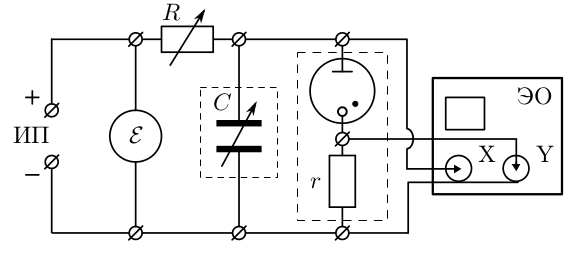
\includegraphics[width=0.5\textwidth]{images/picture_4.png}
        \captionof{figure}{Схема установки для исследования релаксационных колебаний}
    \end{center}
    Схема экспериментальной установки представлена на рис. 4. Штриховой линией на схеме выделена 
    панель, на которой установлены газонаполненный диод (стабилитрон) и последовательно с ним 
    резистор $r$, позволяющий предохранить этот диод от перегорания, а также по напряжению на нём
    измерить ток разряда. Этот резистор остаётся включённым при всех измерениях. Это означает, что
    во всех написанных выше формулах под $R$ нужно понимать $R + r$.

    Добавочное сопротивление газоразрядной лампы в установке, за которой выполнялась работа равно:
    \[r = 5.1 кОм\]

\section{Измерения и обработка их результатов}

    \subsection{ВАХ стабилитрона}

    Для установления вольт-амперной характеристики газоразрядного диода была собрана следующая схема:
    \begin{center}
        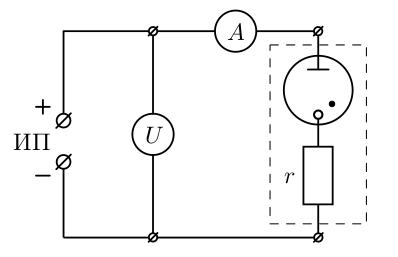
\includegraphics[width=0.5\textwidth]{images/picture_5.png}
        \captionof{figure}{Схема установки для исследования ВАХ стабилитрона}
    \end{center}
    Было проведено 27 измерений тока при различных напряжениях. Результаты приведены в таблицах 1 и 2.
    По этим результатам построены график 1 и график 2, на которых отражены зависимости $I(U)$ и $I(U - U_r)$,
    где $U_r = Ir$ - падение напряжения на добавочном сопротивлении.

    Из данных результатов можно заключить, что напряжения зажигания и гашения равны соответственно:
    \[U_1 = (88.7 \pm 0.5) В\ \ и\ \ U_2 = (75.0 \pm 0.5) В\]

    \subsection{Осциллограмма релаксационных колебаний}

    Для исследования осциллограммы над цепь подавалось напряжение $\mathcal{E} \approx 1.2 U_1 = (107.8 \pm 0.5) В$,
    на магазине сопротивлений было выставлено $R = 900\ кОм$, ёмкость конденсатора составила $C = 50 нФ$. 
    Частота развёртки осциллографа подбиралась таким образом, чтобы на экране оказалась картина пилообразных колебаний. 
    По этой картине были оценены величины $\tau_{ch}$ и $\tau_{disch}$:
    \[\tau_{ch} = 16.4\ мс;\ \ \ \tau_{disch} = 0.8\ мс\]
    Таким образом,  
    \[\frac{\tau_{ch}}{\tau_{disch}} \approx 20.5; \ \ \ T = 17.2\ мс; \ \ \ \nu \approx 5.81 кГц\]

    Далее проводилось последовательное уменьшение сопротивления магазина с целью определения критического
    сопротивления $R_{кр}$, при котором колебания уже невозможны. В ходе работы удалось получить значение:
    \[R_{кр} = 129\ кОм\]

    Для определения периода релаксационных колебаний было проведено две серии измерений. В первой на магазине
    сопротивлений было выставлено $R = 400\ кОм$, при этом ёмкость конденсатора менялась от 50 нФ до 2 нФ. Во
    второй серии была установлена постоянная ёмкость $C = 50 нФ$, а сопротивление магазина менялось от 900 кОм
    до 130 кОм. Для каждой из этих серий были определены период и частота релаксационных колебаний. Результаты
    приведены в таблицах 3 и 4 вместе с теоретическим значениями для периодов и частот, полученными по формуле
    \eqref{period}. По данным этих таблиц также построены графики. Видим, что графики отличаются незначительно.

\section{Вывод}

    В ходе работы исследованы релаксационные колебания в вырожденной автоколебательной системе, содержащей
    газоразрядную лампу. Получена качественная картина зависимости напряжения от времени с помощью осциллографа,
    а также найдены зависимости периода таких колебаний от параметров электрической цепи.

\newpage
\section{Приложения}

    \subsection{Таблицы}

    \begin{minipage}{0.49\linewidth}
    \begin{center}
    \captionof{table}{ВАХ при возрастании напряжения}
        \begin{tabular}{|c|c|c|c|c|}
            \hline
            U, В    & $U - U_r$, В & $\sigma_U$, В         & I, мА & $\sigma_I$, мА        \\ \hline
            \hline
            0       & 0          & \multirow{16}{*}{0.5} & 0     & \multirow{16}{*}{0.5} \\ \hhline{--~-~}
            12.16   & 12.16      &                       & 0     &                       \\ \hhline{--~-~}
            30.6    & 30.6       &                       & 0     &                       \\ \hhline{--~-~}
            50.0    & 50         &                       & 0     &                       \\ \hhline{--~-~}
            68.5    & 68.5       &                       & 0     &                       \\ \hhline{--~-~}
            80.8    & 80.8       &                       & 0     &                       \\ \hhline{--~-~}
            88.7    & 72.89      &                       & 3.1   &                       \\ \hhline{--~-~}
            99.1    & 74.11      &                       & 4.9   &                       \\ \hhline{--~-~}
            111.3   & 75.09      &                       & 7.1   &                       \\ \hhline{--~-~}
            120.4   & 75.265     &                       & 8.85  &                       \\ \hhline{--~-~}
            129.9   & 74.106     &                       & 10.94 &                       \\ \hhline{--~-~}
            140.4   & 74.61      &                       & 12.9  &                       \\ \hhline{--~-~}
            150.3   & 74.82      &                       & 14.8  &                       \\ \hhline{--~-~}
            160.8   & 75.12      &                       & 16.8  &                       \\ \hhline{--~-~}
            170.0   & 75.65      &                       & 18.5  &                       \\ \hhline{--~-~}
            177.0   & 75.51      &                       & 19.9  &                       \\ \hline
        \end{tabular}
    \end{center}
    \end{minipage}
    \hfill
    \begin{minipage}{0.49\linewidth}
    \begin{center}
        \captionof{table}{ВАХ при уменьшении напряжения}
        \begin{tabular}{|c|c|c|c|c|}
            \hline
            U, В    & $U - U_r$, В & $\sigma_U$, В         & I, мА & $\sigma_I$, мА     \\ \hline
            \hline
            171.0   & 75.63     & \multirow{11}{*}{0.5} & 18.7  & \multirow{11}{*}{0.5} \\ \hhline{--~-~}
            160.8   & 75.12     &                       & 16.8  &                       \\ \hhline{--~-~}
            146.1   & 74.70     &                       & 14    &                       \\ \hhline{--~-~}
            136.0   & 74.29     &                       & 12.1  &                       \\ \hhline{--~-~}
            125.8   & 73.78     &                       & 10.2  &                       \\ \hhline{--~-~}
            114.1   & 73.81     &                       & 7.9   &                       \\ \hhline{--~-~}
            106.0   & 73.87     &                       & 6.3   &                       \\ \hhline{--~-~}
            95.4    & 72.96     &                       & 4.4   &                       \\ \hhline{--~-~}
            84.8    & 72.05     &                       & 2.5   &                       \\ \hhline{--~-~}
            80.5    & 71.83     &                       & 1.7   &                       \\ \hhline{--~-~}
            75.0    & 75.00     &                       & 0     &                       \\ \hline
        \end{tabular}
    \end{center}
    \end{minipage}

    \begin{center}
        \captionof{table}{T(C) при R = const}
        \begin{tabular}{|c|c|c|c|c|}
            \hline
            C, нФ & T, мс & $\nu$, кГц & $T^{(теор)}$, мс & $\nu^{(теор)}$, кГц \\ \hline
            \hline
            50    & 7.6   &  132       & 10.8 & 92   \\ \hline
            44    & 6.6   &  152       & 9.5  & 105  \\ \hline
            38    & 5.7   &  175       & 8.2  & 122  \\ \hline
            32    & 4.6   &  217       & 6.9  & 144  \\ \hline
            26    & 3.7   &  270       & 5.6  & 178  \\ \hline
            20    & 2.7   &  370       & 4.3  & 231  \\ \hline
            14    & 1.75  &  571       & 3.0  & 330  \\ \hline
            8     & 0.95  &  1053      & 1.7  & 578  \\ \hline
            2     & 0.25  &  4000      & 0.4  & 2310 \\ \hline
        \end{tabular}
    \end{center}

    \begin{center}
        \captionof{table}{T(R) при C = const}
        \begin{tabular}{|c|c|c|c|c|}
            \hline
            R, кОм & T, мс & $\nu$, кГц & $T^{(теор)}$, мс & $\nu^{(теор)}$, кГц    \\ \hline
            \hline
            900    & 18.0  & 56         & 24.3  & 41  \\ \hline
            800    & 15.6  & 64         & 21.6  & 46  \\ \hline
            700    & 13.6  & 74         & 18.9  & 53  \\ \hline
            600    & 11.6  & 86         & 16.2  & 62  \\ \hline
            500    & 9.8   & 102        & 13.5  & 74  \\ \hline
            400    & 7.8   & 130        & 10.8  & 92  \\ \hline
            300    & 5.6   & 190        &  8.1  & 123 \\ \hline
            200    & 3.6   & 280        &  5.4  & 185 \\ \hline
            150    & 2.4   & 420        &  4.1  & 247 \\ \hline
            130    & 1.7   & 590        &  3.5  & 285 \\ \hline       
        \end{tabular}
    \end{center}

    \newpage
    \subsection{Графики}

    \textbf{График 1. $I(U),\ I(U - r)$ при увеличении напряжения}
    \begin{center}
        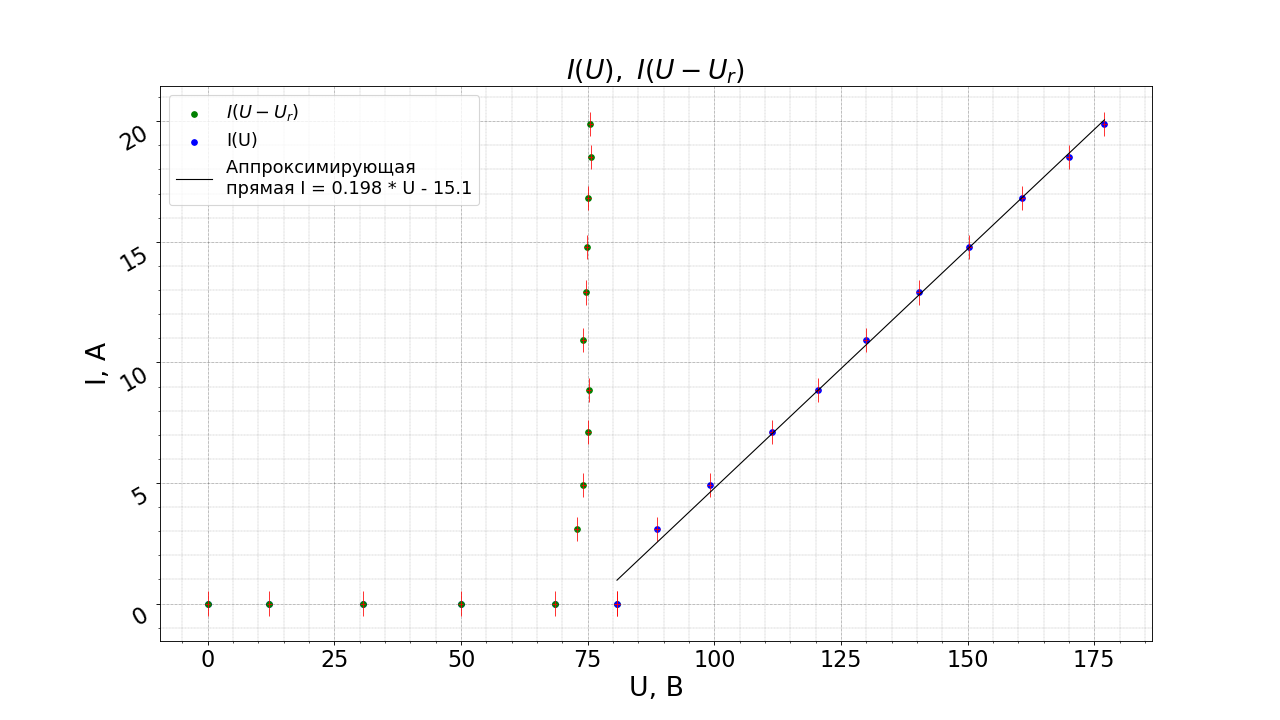
\includegraphics[width=\textwidth]{images/graph_1.png}
    \end{center}

    \textbf{График 2. $I(U),\ I(U - r)$ при уменьшении напряжения}
    \begin{center}
        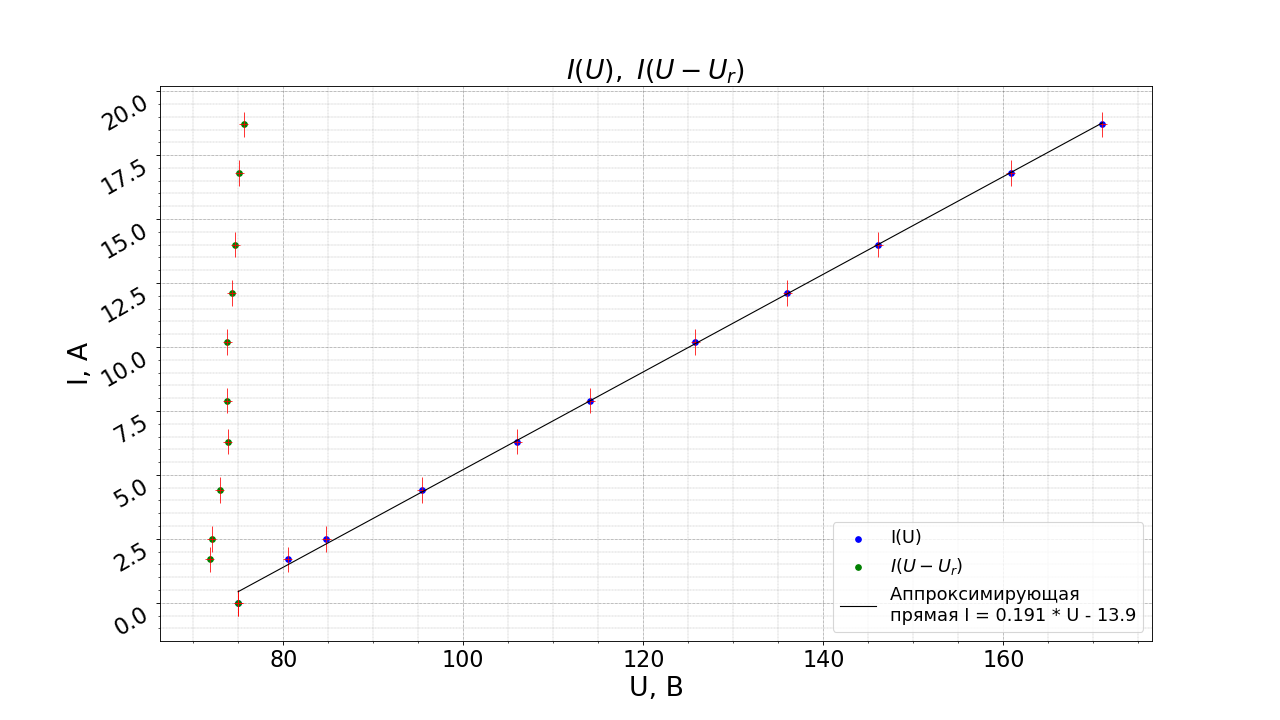
\includegraphics[width=\textwidth]{images/graph_2.png}
    \end{center}

    \newpage
    \textbf{График 3. T(C) при R = const}
    \begin{center}
        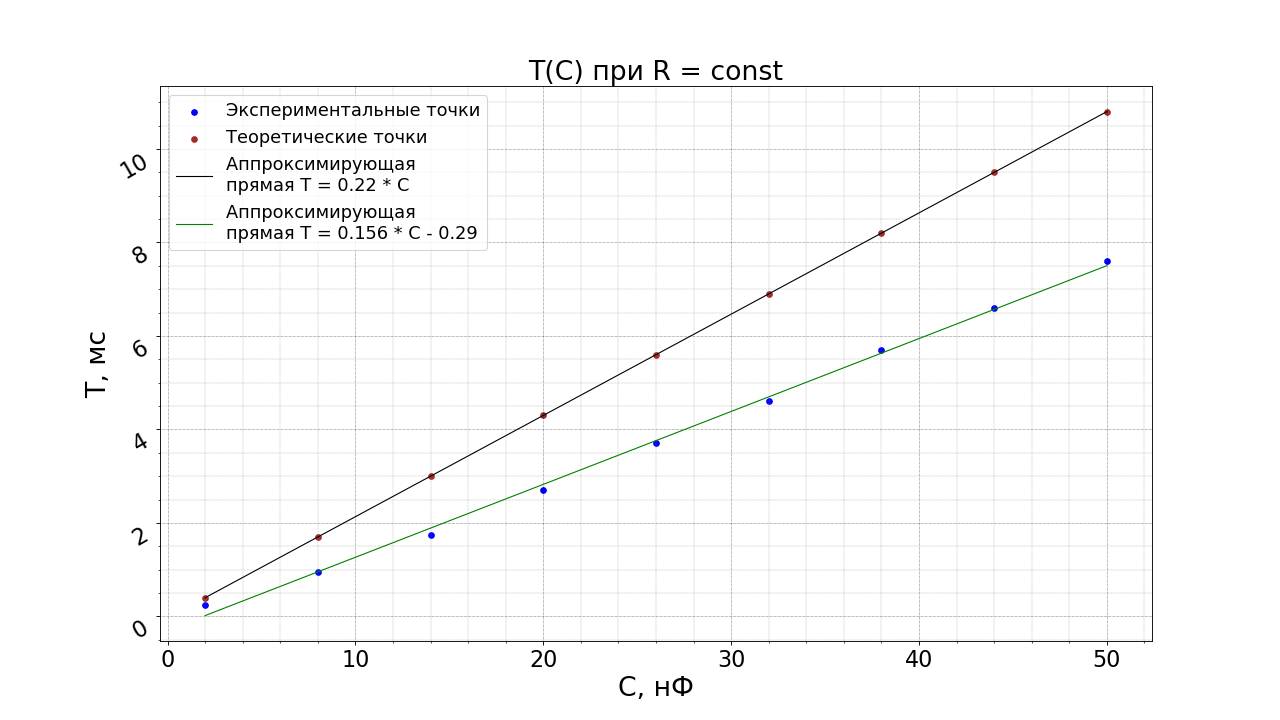
\includegraphics[width=\textwidth]{images/graph_3.png}
    \end{center}

    \textbf{График 4. T(R) при C = const}
    \begin{center}
        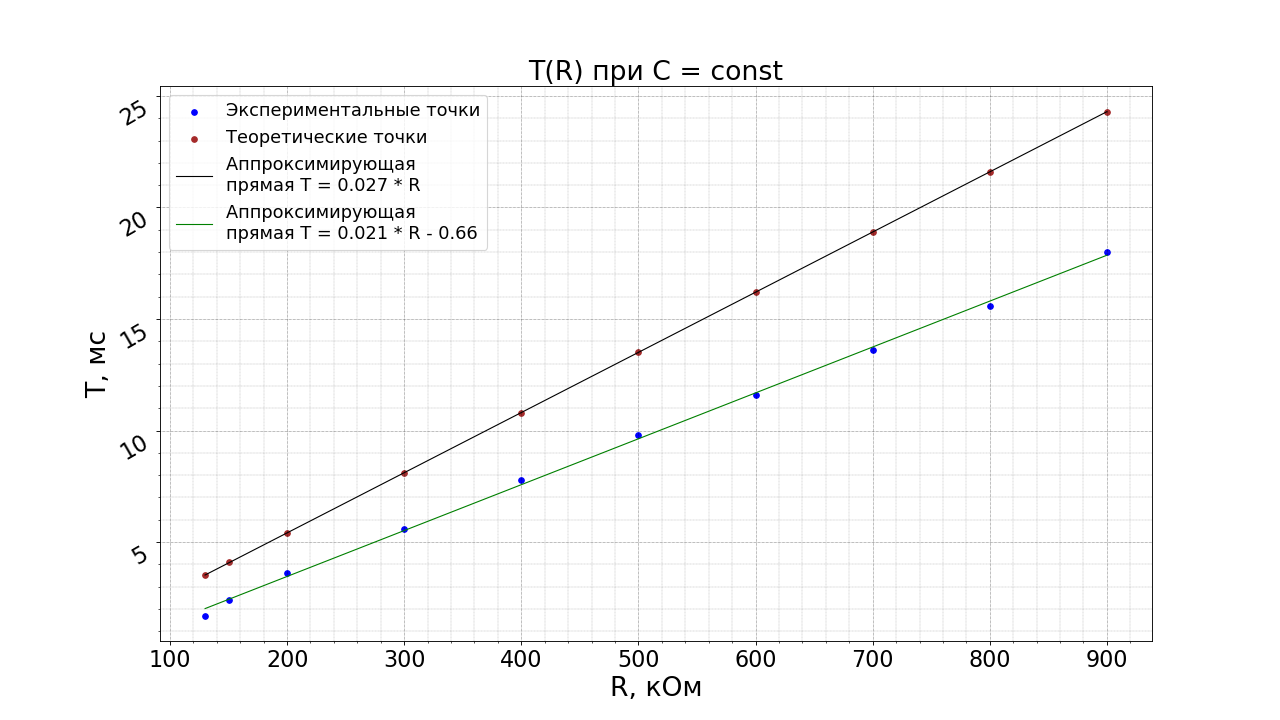
\includegraphics[width=\textwidth]{images/graph_4.png}
    \end{center}

\end{document}
